%!TEX root = ../Thesis.tex
\chapter{Introduction}
\label{sec:intro}

%--------------------------------------------------------------------------------
\clearpage
\section{Energy generation from the wind}
\label{sec:intro_engen}


%--------------------------------------------------------------------------------
\subsection{Motivation and global status}
\label{sec:intro_history}

Global energy systems are currently undergoing a revolution. The production of electricity for household and industrial use has, until the recent past, relied almost entirely on non-renewable fuel sources including coal and petroleum derivatives which are burned to run steam turbine generators. A number of compelling motives exist which are precipitating change to the status quo.

The first motivation being the overwhelming scientific evidence of the impacts of large scale releases of air pollutants into the environment. Particulates have been closely linked to lung (\cite{hamra_outdoor_2014}) and heart disorders (\cite{du_air_2016}). Carbon dioxide, a greenhouse gas, is also released through the combustion process and acts to increase the Earth's surface temperature through radiative forcing (\cite{charlson_climate_1992}), as well as acidify water bodies through the formation of carbonic acid and harming marine life (\cite{doney_ocean_2009}). Other pollutants including sulfur oxides and nitrogen oxides contribute to smog and acid rain, and are similarly linked to acute heath effects (\cite{brunekreef_air_2002}).

Realizing the urgency of these environmental concerns, authorities across the world have begun to enact agreements to curb their emissions contributions. These pacts can range from city and regional planning regulations, to national legislation and international treaties. Examples include the United Nations Kyoto Protocol and Paris Climate Agreement, European Commission's Clean Energy for all Europeans Framework (\cite{ec_clean_energy}), China's Renewable Portfolio Standard (\cite{china_rps}) and Denmark's Energy Strategy (\cite{danmark_energi}). In conjunction with improvements in energy efficiency, large impacts can be made by the exchange and supplementation of low-carbon, renewable based generation including wind and solar.

Beyond commitments to avoiding the negatives associated with hydrocarbon based fuels, new opportunities have emerged with the maturation specifically of the wind energy industry. Rapid cost decreases have been demonstrated through experience, competition, and scaling which have brought the levelized-cost-of-energy (LCOE) of onshore wind power within reach and in many areas below that of traditional power plants without the need for subsidies. The IRENA renewable cost database reveals a 2017 average global LCOE for onshore wind at 60 and offshore wind at 140 USD/MWh, with projections for further decreases in the coming years (\cite{IRENA_2018}). The 2019 tender for Saudi Arabia's first installation, the 400 MW Dumat Al Jandal wind farm, resulted in a record power purchase agreement (PPA) of 21.3 USD/MWh (\cite{masdar_edf_2019}).

\begin{comment}
    An additional compelling reason to...
    <geopolitical motivations from o and g from the middle east, Russia, etc.
    security of supply for self-sufficiency>
\end{comment}

While wind power only supplies about 4\% of global electricity demand at present, the aforementioned developments have resulted in a large and rapid expansion of planned and installed projects worldwide. Figure \ref{fig:wind_power_cum} presents a timeline of cumulative globally installed wind power, with the 2017 aggregate totalling over 539 GW. The growth rate is projected to remain near 10\%, year on year (\cite{gwec_global_2017}).

\begin{figure}[htbp]
    \centering
        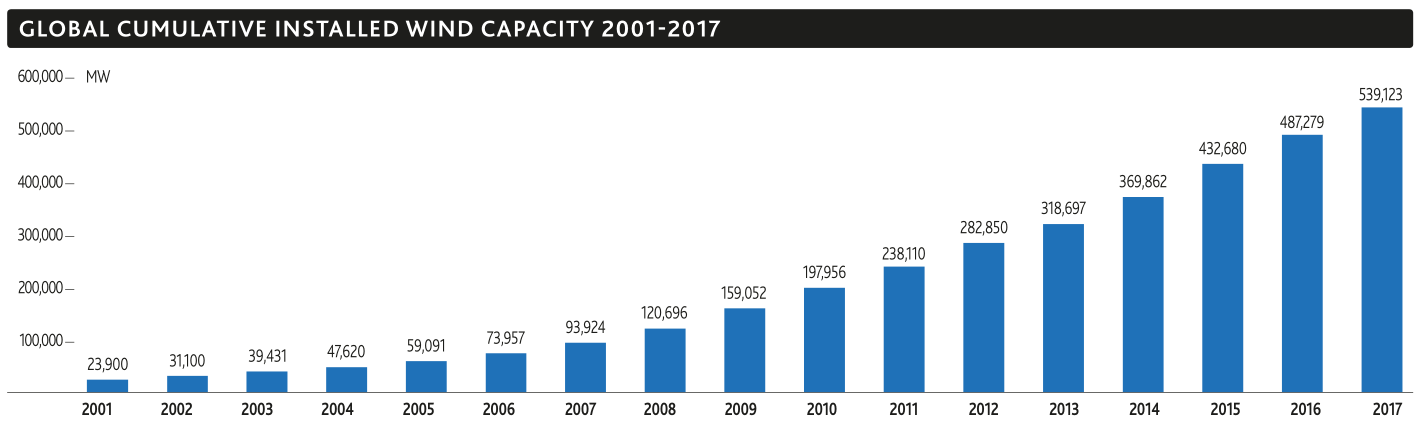
\includegraphics[width=1.0\textwidth]{graphics/intro/motivation_market/wind_power_cum.png}
    \caption{Cumulative worldwide installed wind power capacity from 2001-2017. The current value exceeding 539 GW. Source: \cite{gwec_global_2017}}
    \label{fig:wind_power_cum}
\end{figure}

%--------------------------------------------------------------------------------
\clearpage
\subsection{Intermittency of wind resource}
\label{sec:intro_intermittency}

The reliable and efficient exploitation of wind power faces a unique set of challenges. Electrical energy produced by wind turbines is derived from the kinetic energy of the wind. Air flow generates a lift force on the blades causing them to rotate. This mechanical energy ultimately drives the generator, producing electricity which is collected and fed to the power grid. As the wind is not a controllable fuel source, the turbine's output will to a large extent be determined by atmospheric conditions.

Winds originate from differential heating of the Earth's surface and are transported by bulk motion. Within the boundary layer, they are largely influenced by the planet's surface (terrain and vegetation), human made obstacles, weather systems, and turbulent mixing.

Wind variability is defined as the fluctuations in energy content of the wind. These variations occur across a wide range of temporal and spatial scales. Contributions can include diurnal, seasonal, and interannual patterns, and physical processes including: gravity waves, cold fronts, storms, cellular convection, convective rolls, low level jets, and sea breezes (\cite{vincent_forecasting_2017}). Combinations of these synoptic-, meso- and micro-scale influences lead to a high degree of intermittency in the wind, as shown in Figure \ref{fig:wind_speed_power_ts} using 1-second measurements.

Analysis of the power spectral density of wind measurements demonstrates the distribution of these energies by frequency. 
An example is shown in Figure \ref{fig:wind_speed_power_psd} using the same high-frequency meteorological and turbine data. The 

\begin{figure}[htbp]
    \centering
        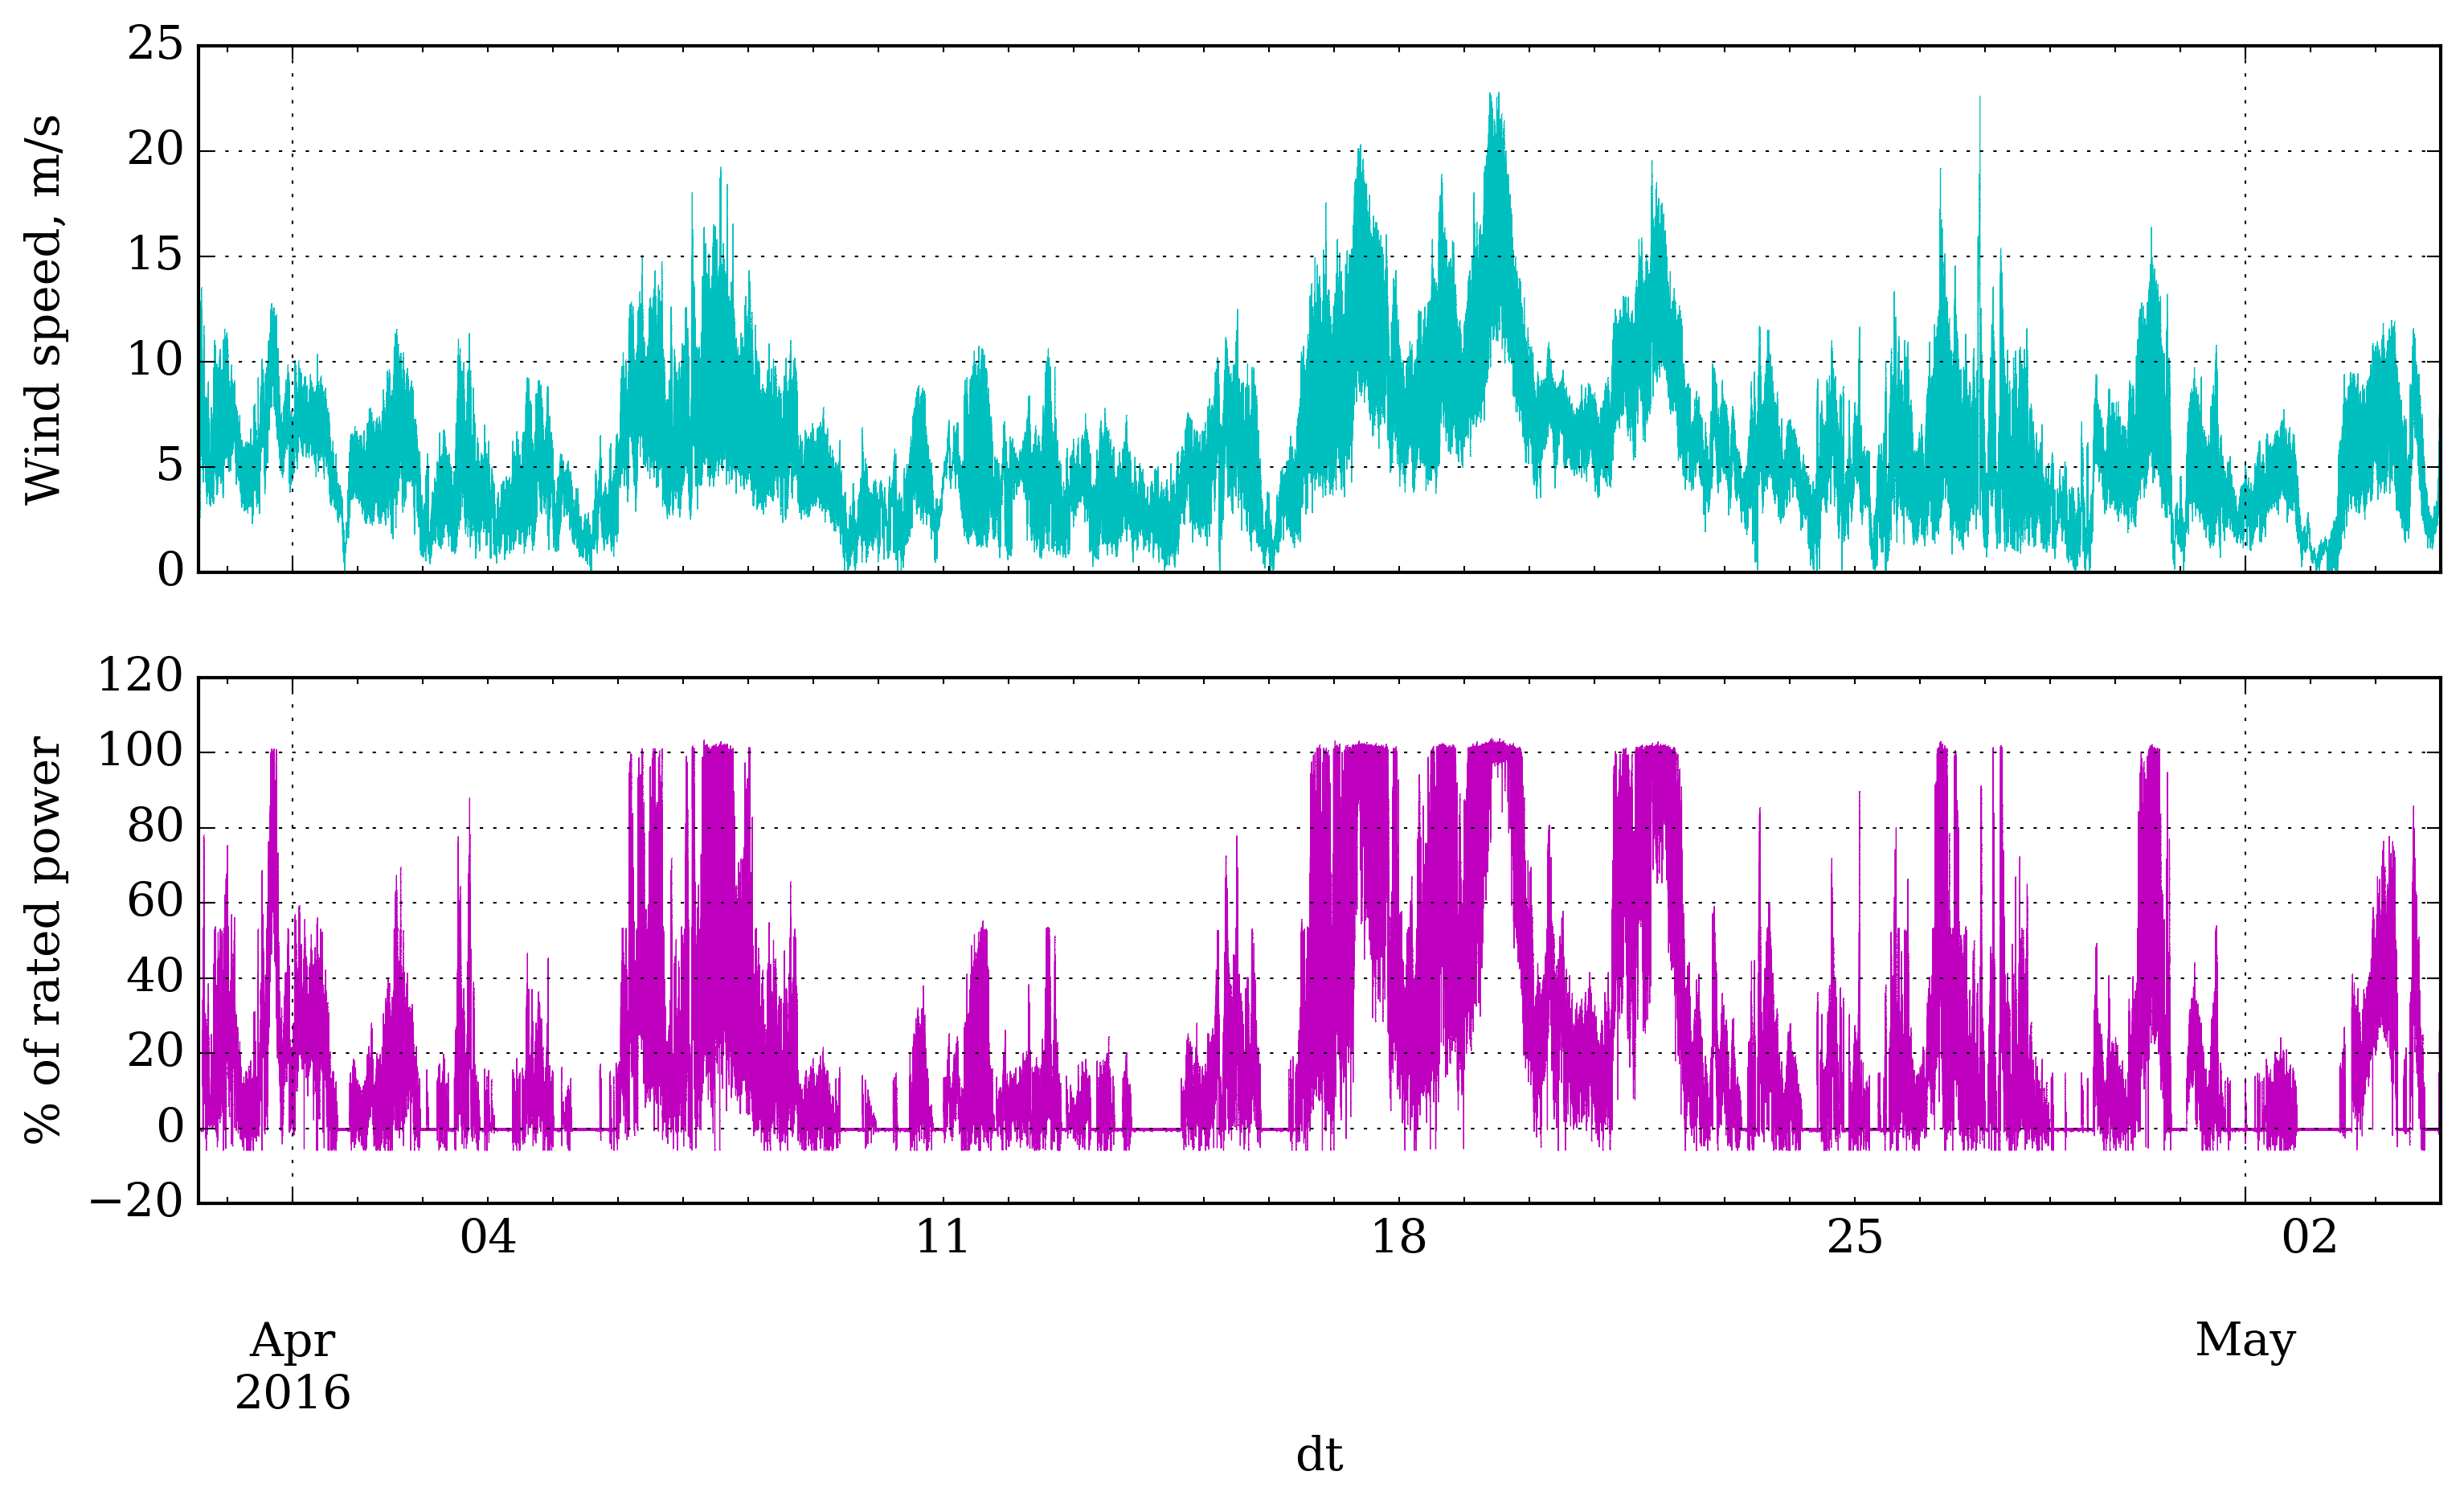
\includegraphics[width=1.0\textwidth]{graphics/intro/variability/wind_speed_power_ts.png}
    \caption{Time series example of wind speed (top) and wind power (bottom) variability from DTU's V52 research turbine}
    \label{fig:wind_speed_power_ts}
\end{figure}

\begin{figure}[htbp]
    \centering
        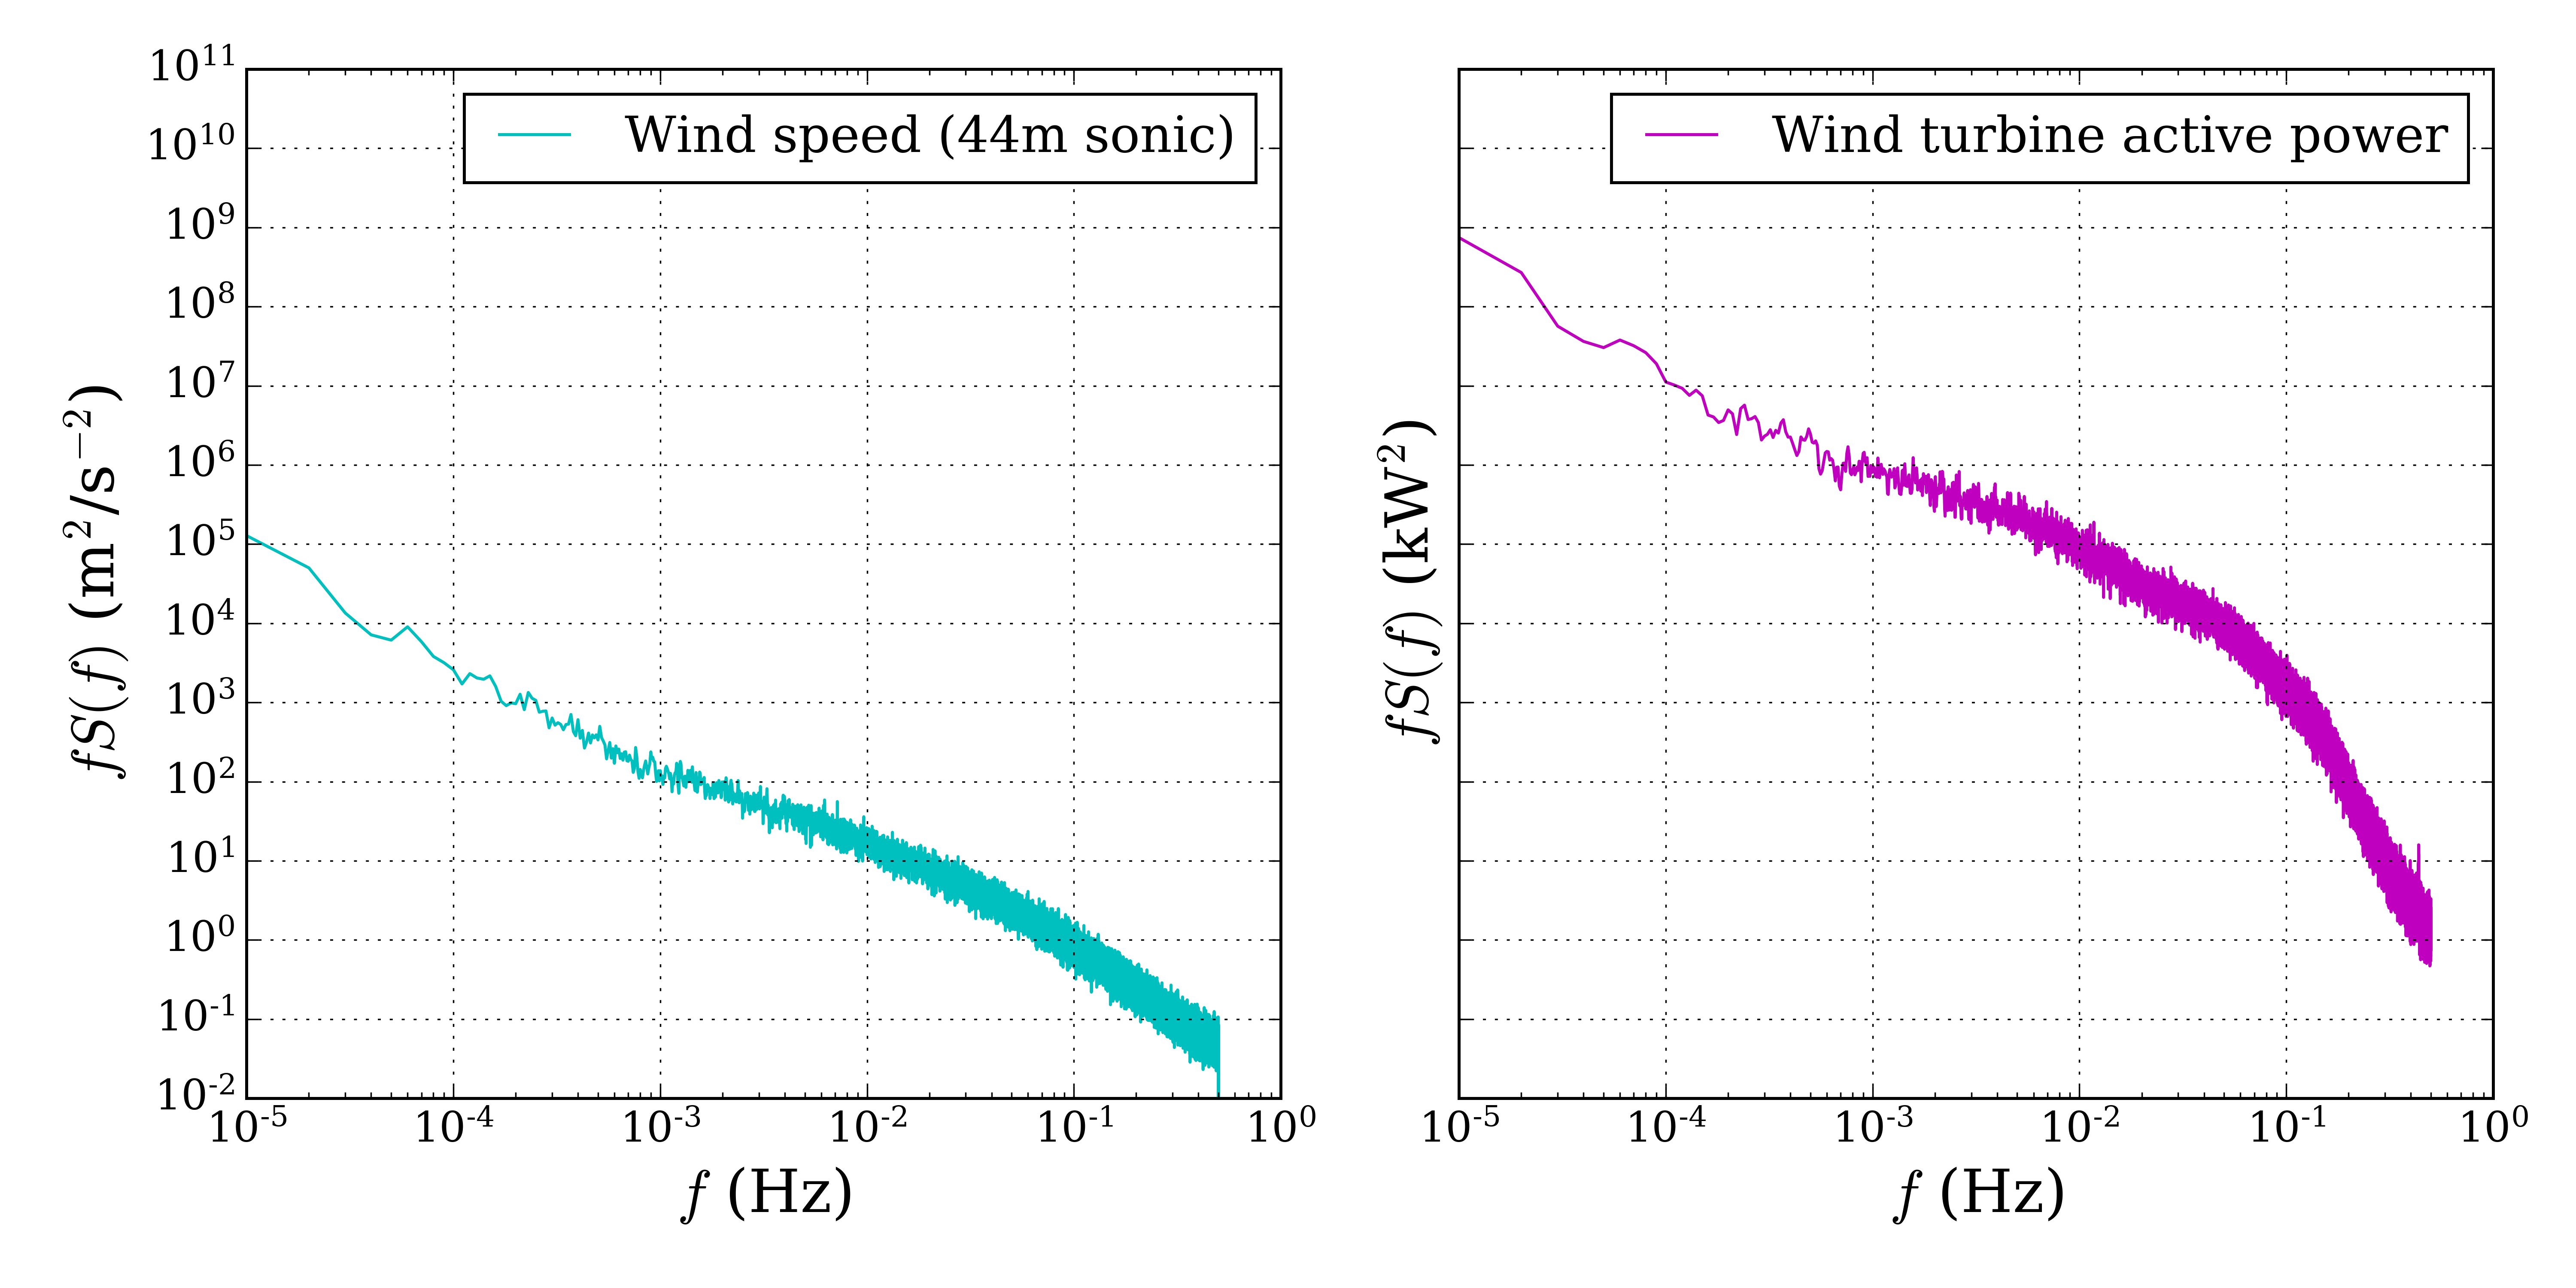
\includegraphics[width=1.0\textwidth]{graphics/intro/variability/wind_speed_power_psd.png}
    \caption{Power spectral density (PSD) comparison between wind speed and wind power from DTU's V52 research turbine}
    \label{fig:wind_speed_power_psd}
\end{figure}

%\cite{larsen_full_scale_2016} 

%The variability of the wind 
%Winds consist of a dominant wind force but also irregular fluctuations (turbulence)
%varying levels of turbulence 
%turbulent kinetic energy (TKE) driven by atmospheric stability
% other interactions such as with thermal convective up/downdrafts and turbulent eddies
%Wind motion exists Global atmospheric circulation originates from differential heating of the Earth's poles and equator which is rotated by the Coriolis force due to the planet's spin. Large scale circulation cells 
%Winds are characterized by their velocity (speed and direction) and 

TODO:
\begin{itemize}
\color{red}
    \item scales, turbulence etc.
    \item power curve
    \item wind ramps
    \item averaging over rotor area and wind farm area (though highly correlated)
    \item the most rapid variations will to some extent be compensated for by the inertia of the wind turbine rotor.
    \item large number of turbines are usually installed within a small geographical area, leading to correlated fluctuations between many turbines
    \item flexible dispatch, higher predicted variability -> more reserve wind power (curtailment)
    \item balancing in high penetration
    \item there are ideas for storage but none implemented at large scale at this time
\end{itemize}

%--------------------------------------------------------------------------------
\clearpage
\subsubsection{Case study of wind turbine power variability}
\label{sec:intro_intermittency_V52}

To further explore wind variability and its impact on power systems, a summary investigation was conducted to characterize changes in electrical power output from a real world wind turbine. The data consists of high-resolution SCADA measurements from DTU's Vestas V52 research turbine at Ris{\o} (\cite{dtu_v52}). This model is one of the most commonly sold turbines worldwide and has a rated capacity of 850 kW. The sourced data spans from March 30 to May 4th, 2016 (35 days) during a calibration period when the turbine's control systems were under normal operation and no aerodynamic modifications were present. 

Measurements of the turbine's active power signal were down-sampled from 35 Hz to 1-second averages, and normalized with respect to rated power (where a value of 100 represents the generator's nameplate capacity). Note that it is possible to have both values below zero (during start up when drawing power from the grid) as well as values above 100 on the short term.

Statistics of absolute changes in the turbine's normalized power output within various time frames ranging from 1-second to 1-hour are presented in the following. Figure \ref{fig:act_pow_change_vioboxplot} presents a combined violin and boxplot across the selected time windows which illustrates statistical properties such as the shape and width of the distributions, quartile positions, median values, and spread of outliers. This is joined with Table \ref{tab:intro_v52_variability_statistics} describing summary statistics.

\begin{figure}[htbp]
    \centering
        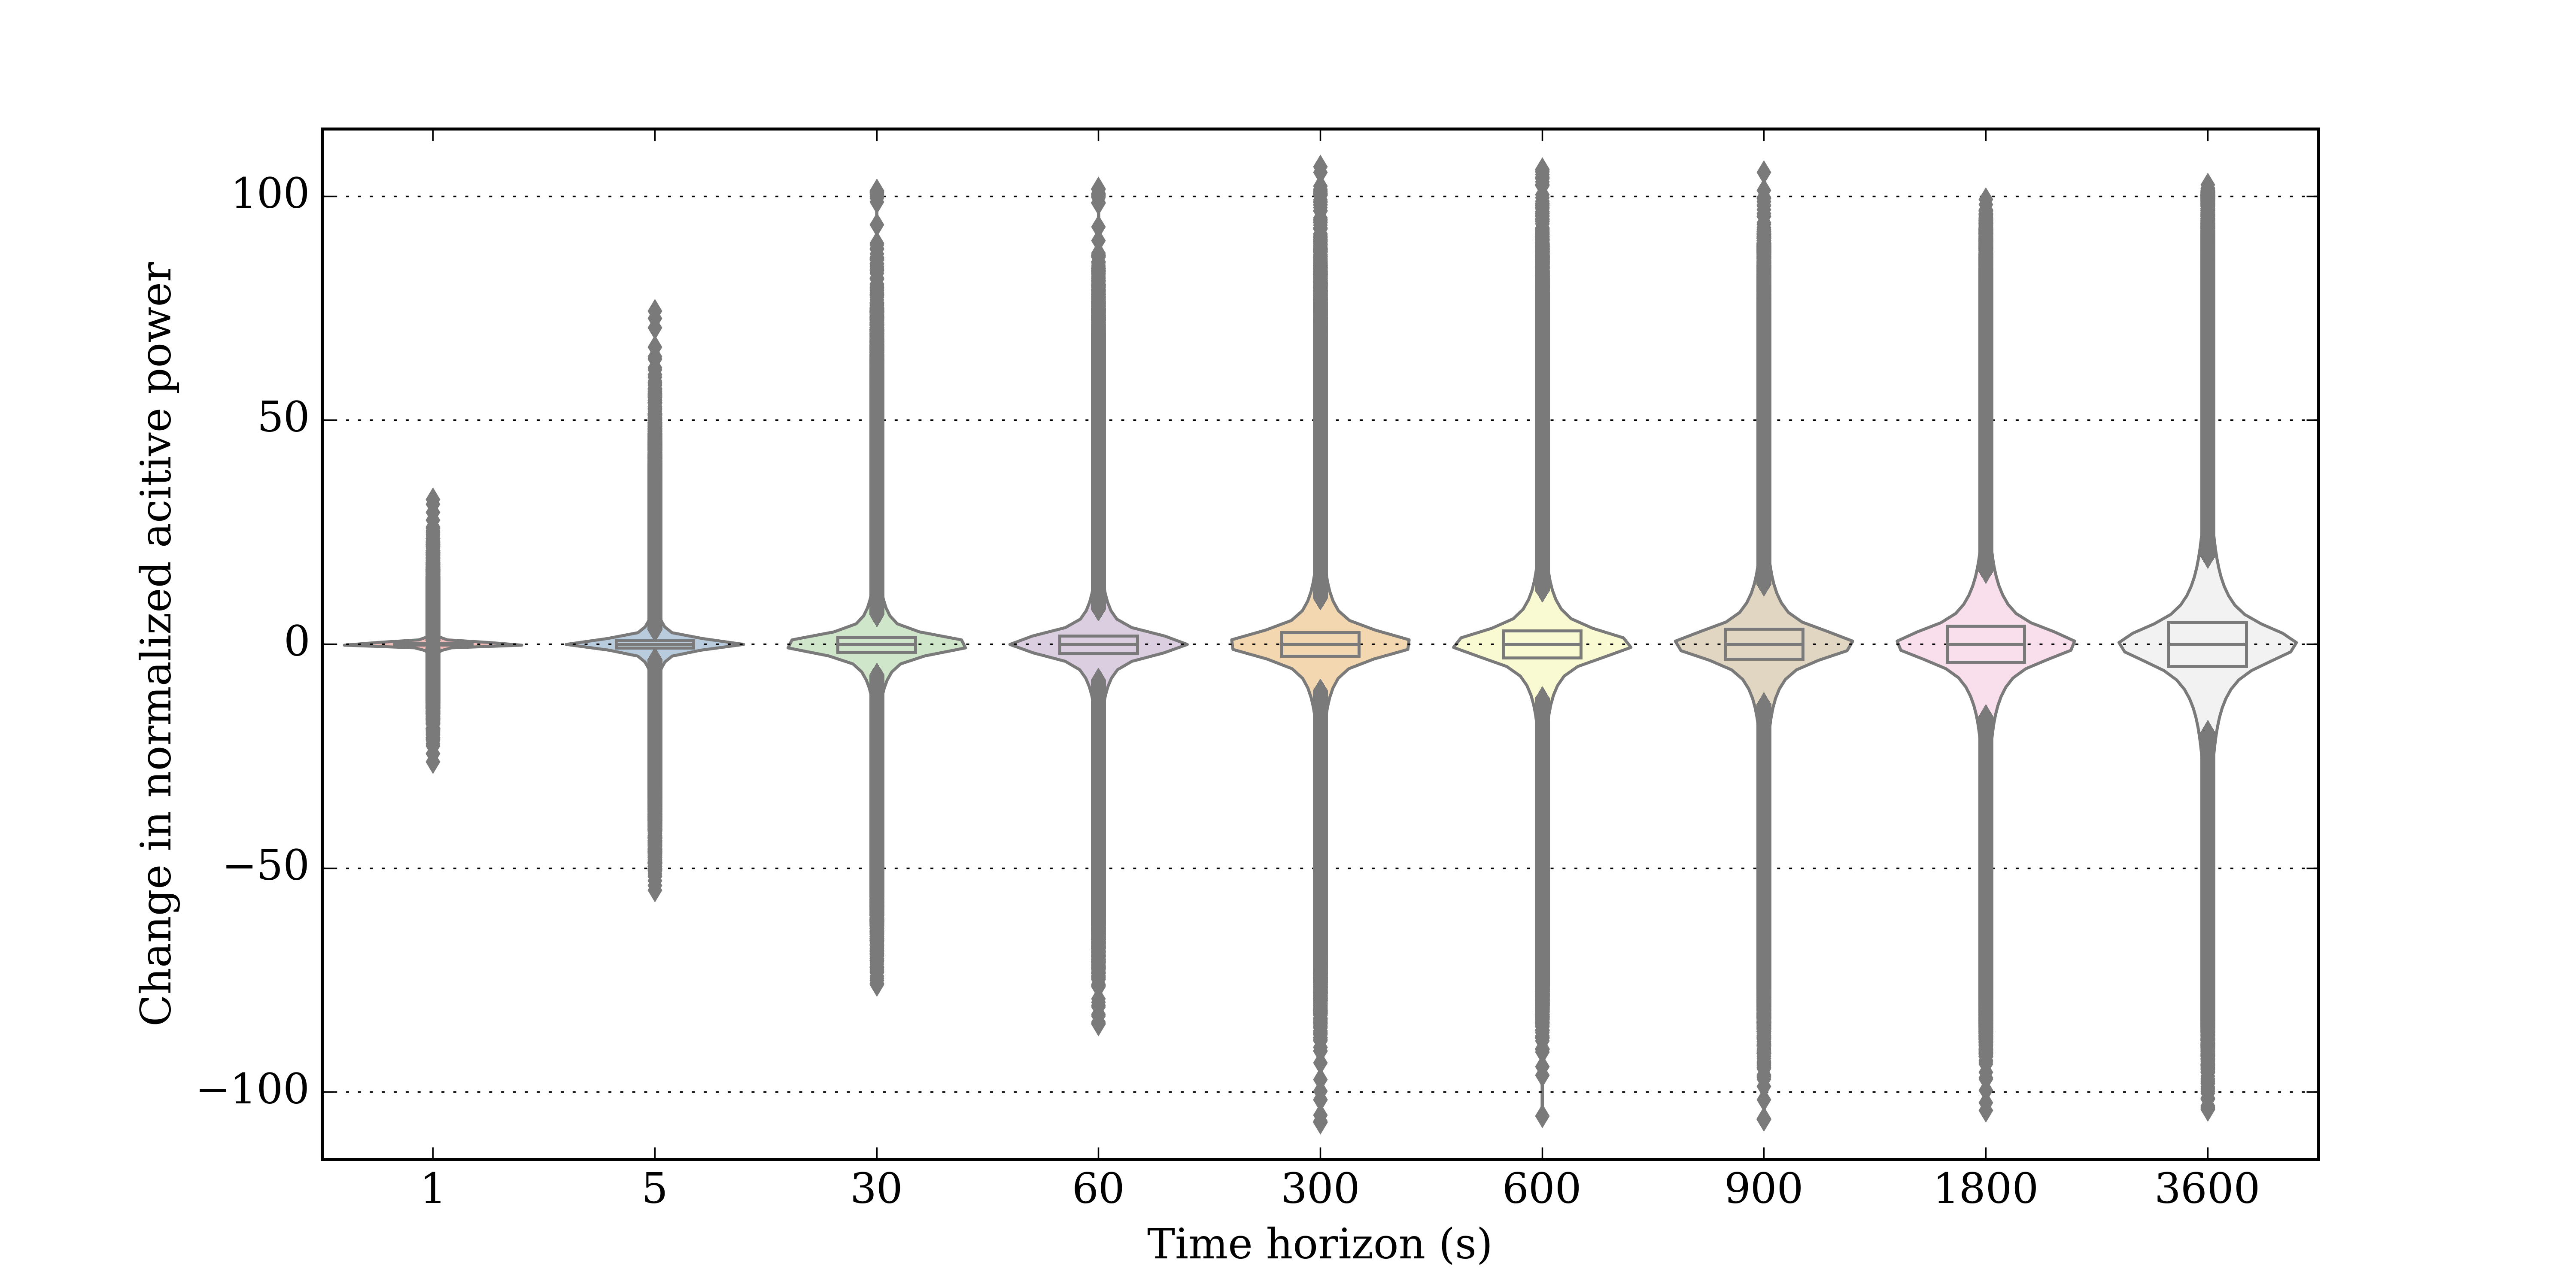
\includegraphics[width=1.0\textwidth]{graphics/intro/variability/act_pow_change_vioboxplot.png}
    \caption{Combined violin and boxplot of normalized active power changes by various time windows from DTU's V52 research wind turbine}
    \label{fig:act_pow_change_vioboxplot}
\end{figure}

\begin{table}
    \centering
    \caption{Table of statistics for V52 power output variability over selected time windows up to 1-hour}
    \resizebox{\columnwidth}{!}{%
\begin{tabular}{lrrrrrrrrr}
\toprule
{} &          1 s &          5 s &         30 s &         60 s &        300 s &        600 s &        900 s &       1800 s &       3600 s \\
\midrule
count &  2976599 &  2976595 &  2976570 &  2976540 &  2976300 &  2976000 &  2975700 &  2974800 &  2973000 \\
mean  &        0.000 &        0.000 &        0.000 &        0.000 &        0.002 &        0.003 &        0.004 &        0.008 &        0.009 \\
std   &        1.209 &        4.387 &        8.133 &        9.536 &       11.362 &       11.976 &       12.532 &       13.674 &       15.485 \\
min   &      -26.250 &      -54.907 &      -76.028 &      -84.816 &     -106.745 &     -105.303 &     -106.126 &     -104.044 &     -103.887 \\
25\%   &       -0.225 &       -0.888 &       -1.841 &       -2.103 &       -2.630 &       -3.075 &       -3.371 &       -4.049 &       -4.957 \\
50\%   &        0.000 &        0.000 &        0.000 &        0.000 &        0.000 &        0.000 &        0.000 &        0.000 &        0.000 \\
75\%   &        0.214 &        0.782 &        1.515 &        1.860 &        2.544 &        2.972 &        3.341 &        4.064 &        4.870 \\
max   &       32.326 &       74.414 &      101.242 &      101.663 &      106.567 &      106.013 &      105.350 &       99.266 &      102.539 \\
\bottomrule
\end{tabular}
}
    \label{tab:intro_v52_variability_statistics}
\end{table}

As expected, the variability grows with the length of the window. In all cases, the mean and median power output change is very close to zero and probability densities are symmetrical (normally distributed). On the very shortest timescales (1 and 5-seconds), the variations within the interquartile range (IQR) are small. However, from 30-seconds to 1-minute windows, the spread grows considerably. By the 5-minute case (300 s), the standard deviation approaches that of the longer timescales.

This is further shown in Figure \ref{fig:norm_act_pow_error_dist}, where the distributions are stacked atop each other for comparison (note the logarithmic y-axis scaling). Tail bumps present for certain time windows near the peripheries indicate periods of automatic start up (right tail) when the cut-in wind speed is reached and shut down (left tail) when the cut-out wind speed is exceeded.

\begin{figure}[htbp]
    \centering
        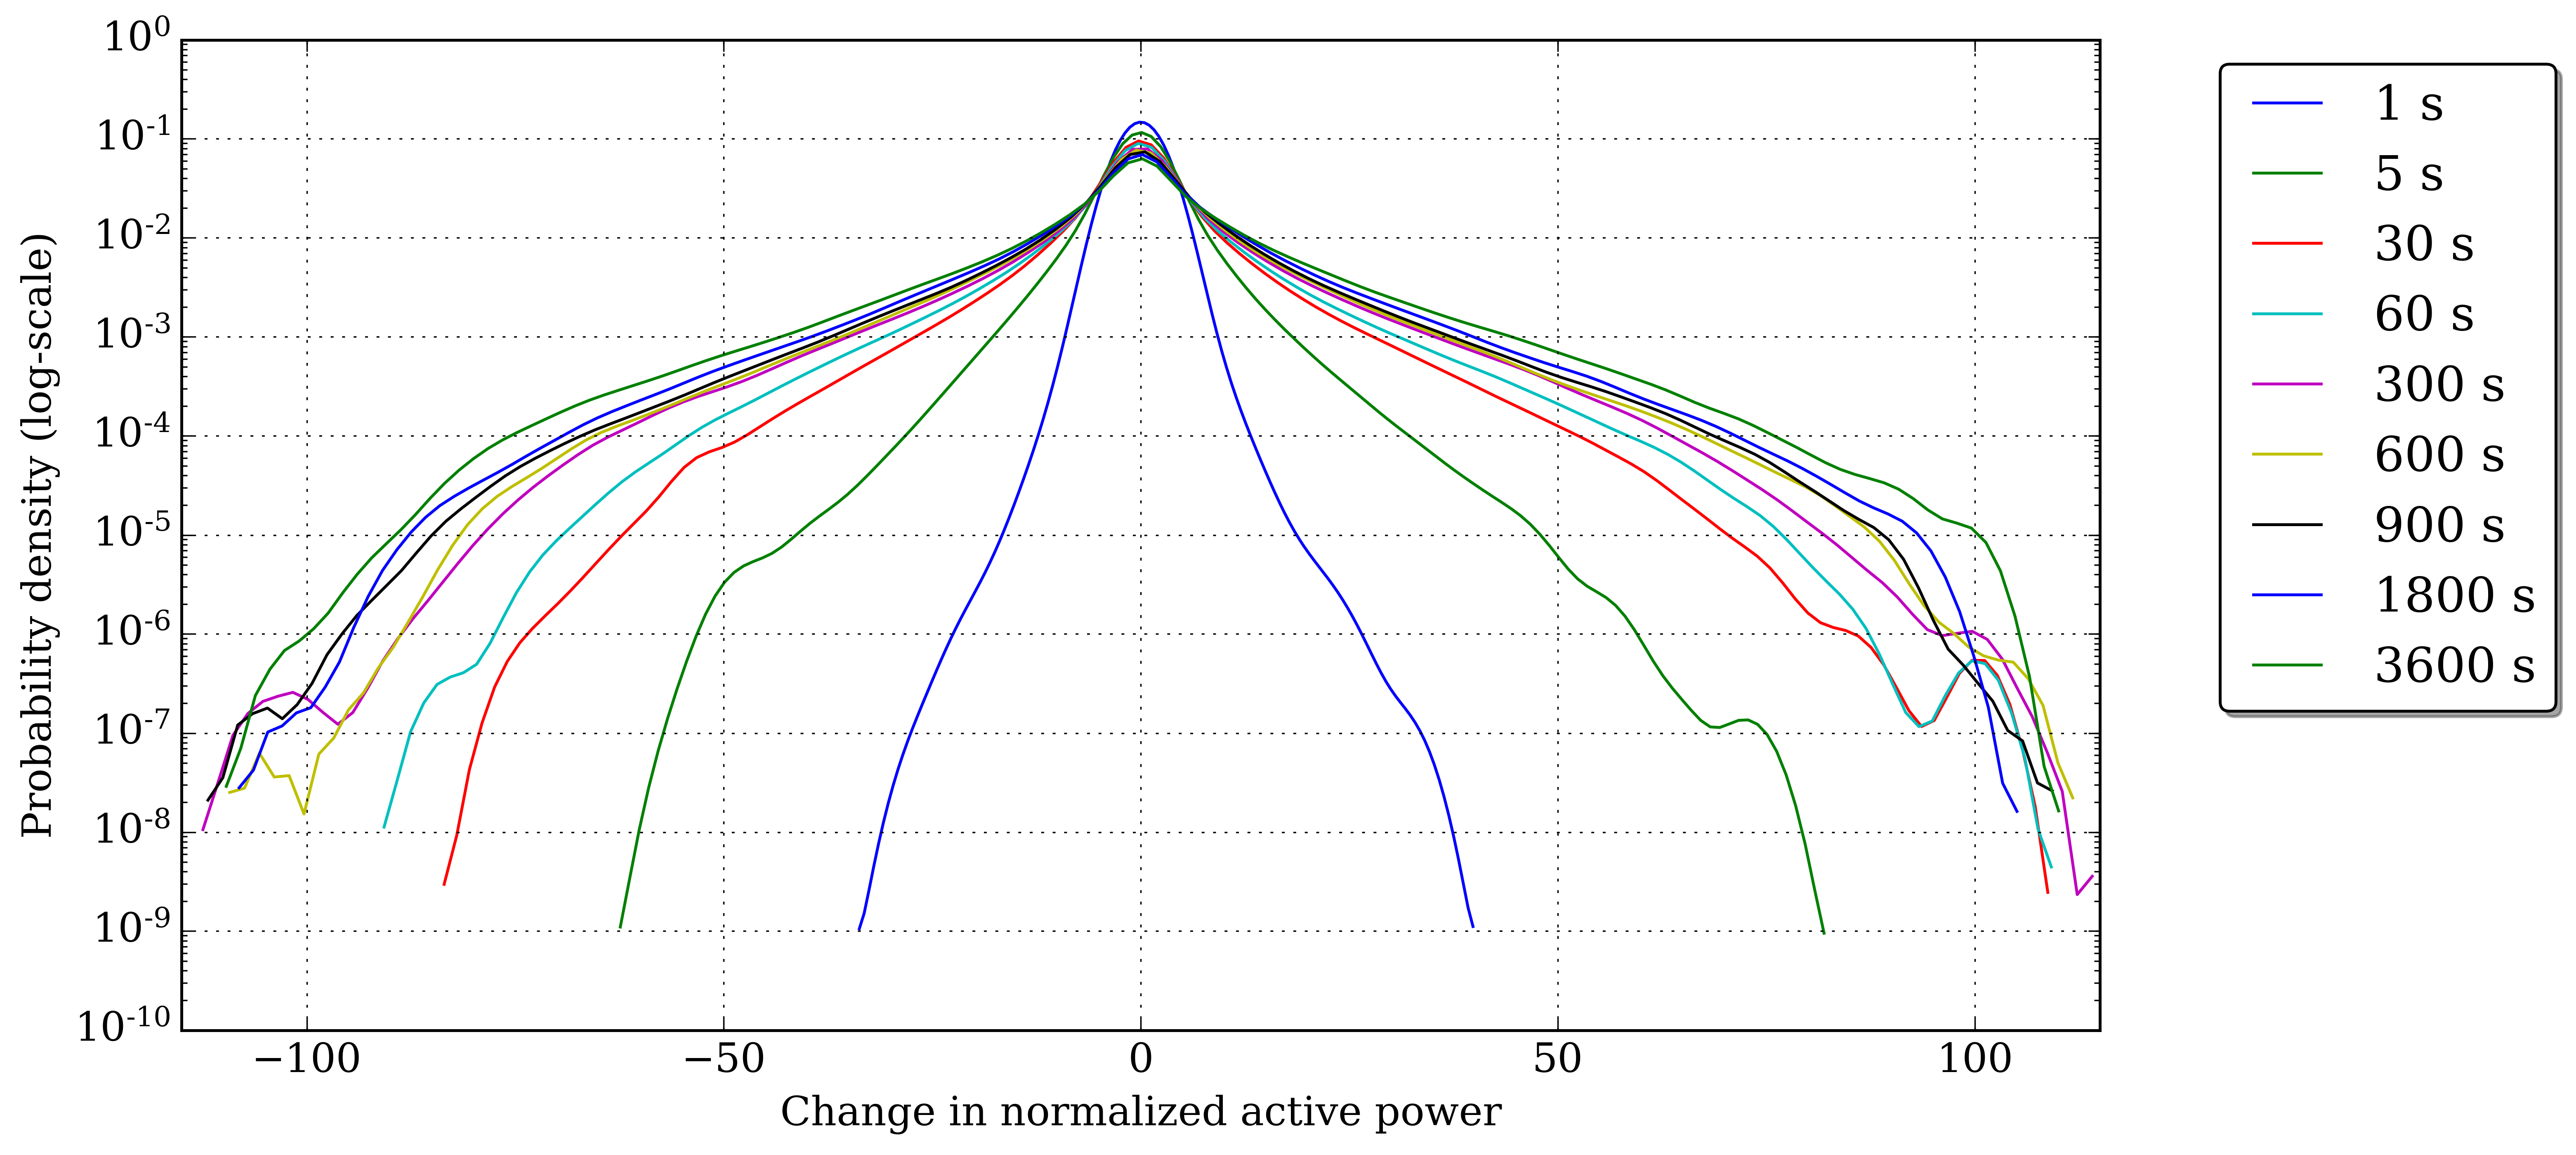
\includegraphics[width=1.0\textwidth]{graphics/intro/variability/norm_act_pow_error_dist.png}
    \caption{Distribution of changes in normalized active power over various time horizons from DTU's V52 research wind turbine}
    \label{fig:norm_act_pow_error_dist}
\end{figure}

This simplified investigation has considered a single wind turbine and not collective wind farm output or otherwise geographically distributed generation which will act to some degree as a smoothing filter. Having said that, the case study has demonstrated that minute-scale variability of wind power is not insignificant and attention should also be focused on this timescale alongside the more commonly focused periods (e.g. 1-hour).

%--------------------------------------------------------------------------------
\clearpage
\subsection{Wind farm control}
\label{sec:intro_control}

TODO:
\begin{itemize}
\color{red}
    \item Farm level control intro
    \item Induction control
    \item Wake steering
\end{itemize}

%--------------------------------------------------------------------------------
\clearpage
\subsection{Forecasting for wind energy}
\label{sec:intro_forecasting}

TODO:
\begin{itemize}
\color{red}
    \item Forecasting intro
    \item Methods (statistical, physical)
    \item Horizon table with common example methods
    \item Evaluating forecasts
\end{itemize}


%--------------------------------------------------------------------------------
\clearpage
\subsection{Power system and electricity markets}
\label{sec:intro_power_markets}

TODO:
\begin{itemize}
\color{red}
    \item Intro to grid design and constraints
    \item Physical balancing
    \item Markets introduction
    \item Economic dispatch
    \item Intrahour market trading
\end{itemize}




\begin{comment}
•	Errors in power forecast do not necessarily reflect impact. Overestimation and underproduction != under prediction and overproduction due to structure of balancing market.
•	The need for spinning reserves. Frequency control/response mode. Droop speed control. Spinning reserve is extremely expensive for utilities. 
•	https://en.wikipedia.org/wiki/Dynamic_demand_(electric_power)#The_need_for_spinning_reserve
•	Cost of imbalance not only money but also CO2
\end{comment}

%--------------------------------------------------------------------------------
%\clearpage
%\subsubsection{Case study of wind power operation in a 5-minute energy market}
%\label{sec:intro_aus_power_study}

%Placeholder for Australian energy market case study


%--------------------------------------------------------------------------------
%--------------------------------------------------------------------------------
\clearpage
\section{Remote sensing}
\label{intro_remote_sensing}

%--------------------------------------------------------------------------------
\subsection{Principles}
\label{sec:intro_rs_principles}

TODO:
\begin{itemize}
\color{red}
    \item Intro
    \item Measurement theory
    \item Introduce lidar and radar
\end{itemize}


%--------------------------------------------------------------------------------
\clearpage
\subsection{Lidar}
\label{sec:intro_lidar}

TODO:
\begin{itemize}
\color{red}
    \item Lidar specific 
    \item Pulsed Doppler lidar measurement chain
    \item Practicalities
    \item Filtering techniques
    \item Interpreting measurements
\end{itemize}


%--------------------------------------------------------------------------------
\clearpage
\subsection{Measurement techniques}
\label{sec:intro_meas_tech}

TODO:
\begin{itemize}
\color{red}
    \item Beam positioning
    \item Switching vs. mechanical
    \item Staring vs. 2D vs. 3D
    \item Fixed vs dynamic trajectories
\end{itemize}

%--------------------------------------------------------------------------------
%\clearpage
%\subsection{Processing, filtering, and interpreting data}
%\label{sec:intro_rs_data}

%TODO:
%\begin{itemize}
%\color{red}
%    \item Data formats
%    \item Filtering techniques
%    \item Interpreting measurements
%\end{itemize}


\clearpage